% 06.1.4. TAREAS Y ESTIMACIONES DE ESFUERZOS POR ITERACIÓN 
%----------------------------------------------------------------------------------------


\paragraph{} Se muestran los esfuerzos previstos para la primera iteración del proyecto en la figura \ref{fig:6141}.

\begin{figure}[h!]
\centering
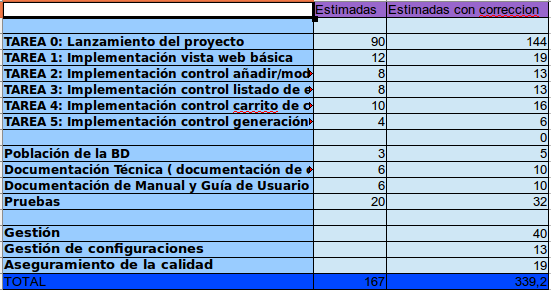
\includegraphics[width=0.95\textwidth]{img/6141}
\caption{Esfuerzos primera iteración}
 \label{fig:6141}
\end{figure}

\paragraph{} Se puede apreciar como la parte más importante de la primera iteración fue el lanzamiento, en el cual se planifico todo el proyecto para concretar todo e intentar evitar posibles problemas. Entre las demás partes se planifico que pruebas, gestión y implementación serías las siguientes tareas más costosas. Esto se puede ver en la~\cref{fig:6142}.

\begin{figure}[h!]
\centering
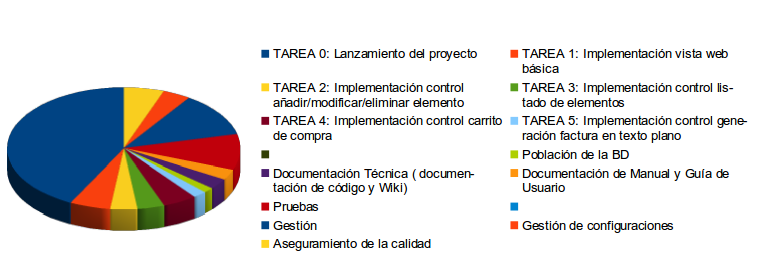
\includegraphics[width=0.95\textwidth]{img/6142}
\caption{Gráfica esfuerzos primera iteración}
 \label{fig:6142}
\end{figure}

\paragraph{} Se muestran los esfuerzos previstos para la segunda iteración del proyecto en la~\cref{fig:6143}. Podemos observar que la mayor parte de horas se la llevan la mejora de la implementación de la interfaz web (con la intención de que la misma tenga un aspecto llamativo y atractivo para el cliente) y las pruebas (con la intención de asegurar completamente que el producto que se le entrega al cliente funciona correctamente en su totalidad). Podemos ver dicho reparto de trabajo más claramente en la~\cref{fig:6144}. 

\begin{figure}[h!]
\centering
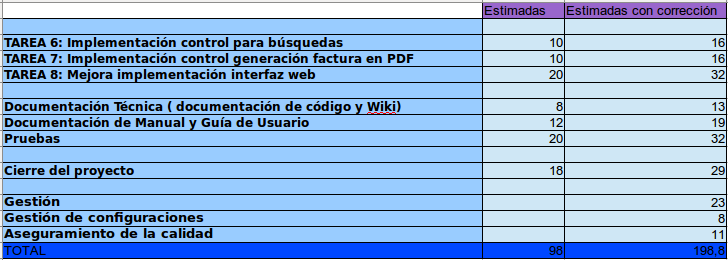
\includegraphics[width=0.95\textwidth]{img/6143}
\caption{Esfuerzos segunda iteración}
 \label{fig:6143}
\end{figure}

\begin{figure}[h!]
\centering
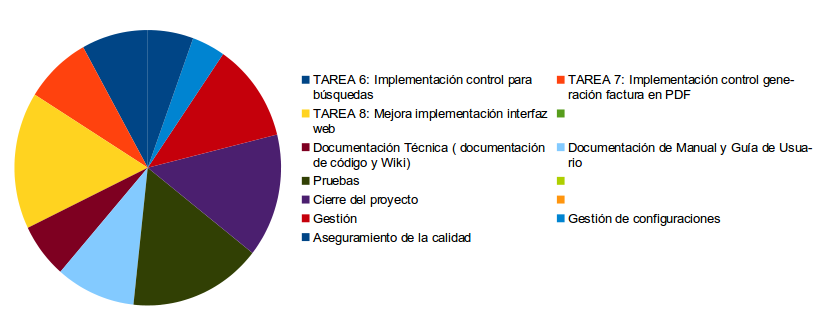
\includegraphics[width=0.95\textwidth]{img/6144}
\caption{Gráfica esfuerzos segunda iteración}
 \label{fig:6144}
\end{figure}